





\newpage
\addtocounter{problemctr}{1}
\noindent
{\bf
Problem \theproblemctr.  (\theinsert \xspace points)}
\swallow{ (\theinserttime\xspace minutes)}

\smallskip

\noindent
Let $L_1$ and $L_2$ be languages.
Let
\(
\mbox{\textit{INSERT}}(L_1, L_2) =
\{w = xyz \mid xz \in L_1 \mbox{ and } y \in L_2\}
\).

\bigskip

\noindent Suppose that $L_1$ and $L_2$ are regular and have the following DFA's:

\bigskip

\begin{figure}[h]
$L_{1}$~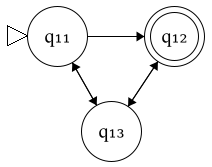
\includegraphics[scale=.5]{dfa1.png}~~~~~~~~~~~~~~~~~~~~~~$L_2$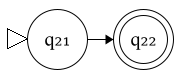
\includegraphics[scale=.5]{dfa2.png}
\centering
\end{figure}


\noindent Below is a partial construction of an NDFA that recognizes $INSERT(L_1,L_2)$. Complete the construction by marking the start state, adding the missing $\epsilon$-transitions, and circling any accept states. \footnote{It turns out you can generalize this procedure to work for any two DFAs. This means that regular languages are closed under the INSERT operation!}

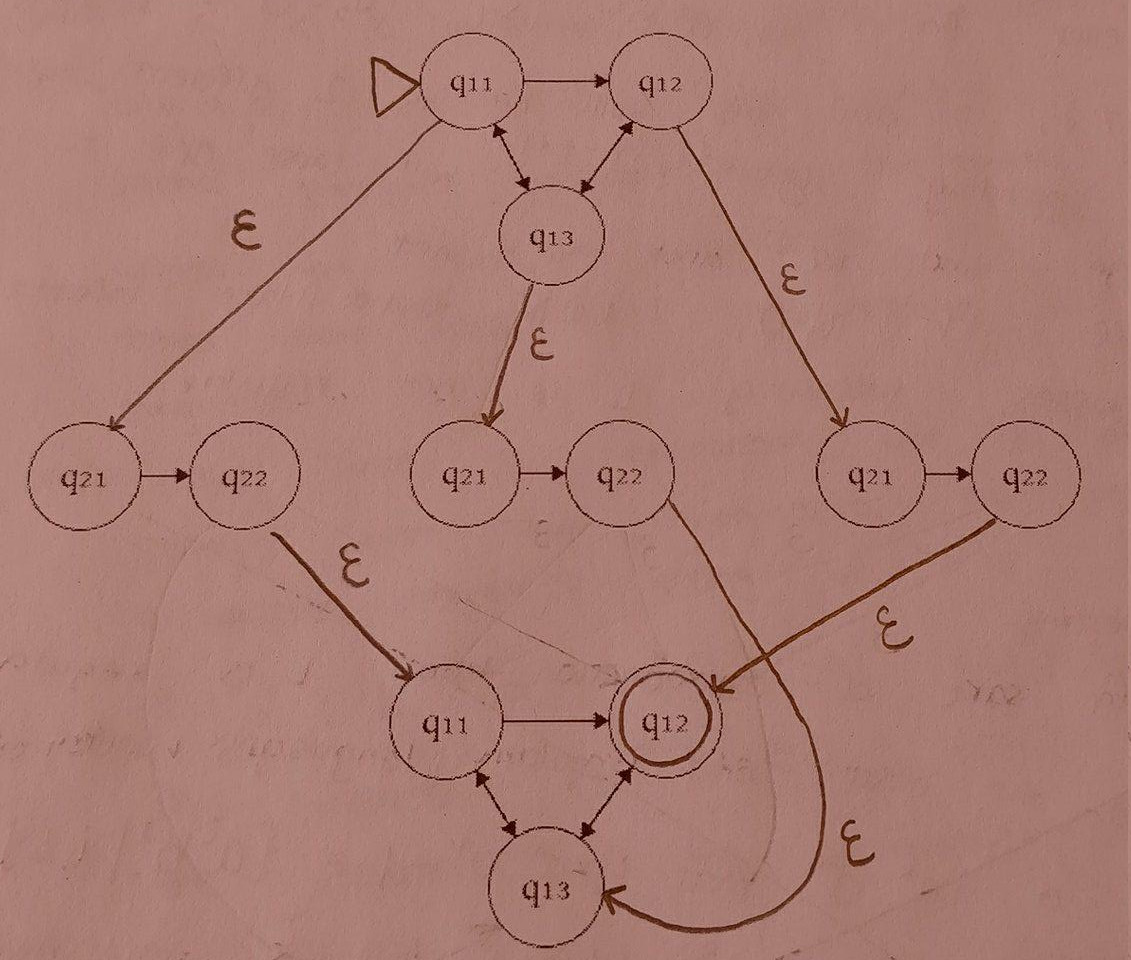
\includegraphics[scale=.4]{insert.jpg}


\iffalse
Using the DFA's for regular languages $L_1$ and $L_2$, this question explores how to construct an NDFA that recognizes $\mbox{\textit{INSERT}}(L_1, L_2)$.

\vspace*{2em}
\noindent
If the DFA for $L_1$ has $k$ states and the DFA for $L_2$ has $\ell$ states, please give your best approximation of the number of states in the NDFA you constructed.

~

\rule{5cm}{.01in}


\bigskip\bigskip\bigskip\bigskip\bigskip

Please try to explain your construction in words \emph{and} with a little sketch.
\fi

